\section{Il progetto di un sistema di controllo in retrazione - Parte 2}

% TODO: non molto soddisfatto di questa sezione !

\subsection{Sintesi in frequenza con la formula di inversione}
% Punti salienti della lezione:
% • Le formule di inversione nel progetto delle reti correttrici con 
% imposizione dei margini di stabilità (margine di fase o di 
% ampiezza)
% • Progetto della rete a ritardo e anticipo e della rete a T con 
% imposizione dei margini di stabilità (margine di fase o di 
% ampiezza)
% • L’equazione diofantea nel progetto del controllore in 
% retroazione con assegnazione arbitraria dei poli retroazionati.


La sintes in frequenza delle reti ritardatici e anticiatrici con imposizione 
di margini di stabilità prestabiliti può essere svolta utilizzando le funzioni 
inverse delle stesse reti.
\subsubsection{Sintesi rete anticipatrice}
Ad esempio una rete anticiatrice:
\begin{equation}
  \frac{1 + j \tau \omega}{1 + j \alpha \tau \omega}
\end{equation}

Il modulo della funzione di trasferimento è:
\begin{equation}
  M = \frac{\sqrt{1 + (\tau \omega)^2}}{\sqrt{1 + (\alpha \tau \omega)^2}}
\end{equation}
Mentre la fase è:
\begin{equation}
  \varphi = \arctan(\tau \omega) - \arctan(\alpha \tau \omega)
\end{equation}

Che permette di riscrivere la formula come:
\begin{equation}
  M e^{j \varphi} = \frac{1 + j \tau \omega}{1 + j \alpha \tau \omega}
\end{equation}

Siano $M, \varphi, \alpha, \omega$ valori reali con $M > 1$ e $\sin \varphi \neq 0$ 
si possono riscrivere le equazioni come:
\begin{equation}
  \begin{cases}
    \alpha = \frac{M \cos \varphi}{M(M - \cos \varphi)} \\
    \omega = \frac{M - \cos \varphi}{\sin \varphi}
  \end{cases}
\end{equation}


La formula di inversione è quindi definita come:
\begin{equation}
  \alpha = \frac{M \cos \varphi - 1}{M(M - \cos \varphi)}, \quad \tau \omega = \frac{M - \cos \varphi}{\sin \varphi}
\end{equation}


Il metodo di sintesi della rete anticipatrice procede come segue:
\begin{enumerate}
  \item Scegliere $\omega_0$ affinchè con  $\varphi_0 := M_F - \arg L(j\omega_0) - \pi$
    valga $\cos \varphi_0 > | L(J\omega_0) |$

  \item Definiti Il modulo e la fase della rete anticiatrice come:
    \begin{equation}
      \begin{cases}
        M = \frac{1}{| L(j\omega_0) |} \\
        \varphi = \varphi_0
      \end{cases}
    \end{equation}
    Uso la formula di inversione per calcolare $\alpha$ e $\tau$.
    \begin{equation}
      \tau = \frac{M - \cos \varphi}{\omega_0 \sin \varphi}
    \end{equation}
    Mentre $\alpha$ è dato da:
    \begin{equation}
      \alpha = \frac{M \cos \varphi - 1}{M(M - \cos \varphi)}
    \end{equation}
\end{enumerate}




\subsubsection{Sintesi rete ritardatrice}
Scegliere $\omega_0$ affinchè con  $\varphi_0 := \arg L(j\omega_0) + \pi - M_F$
valga $\cos \varphi_0 > \frac{1}{| L(J\omega_0) |}$.

Una volta definiti il modulo e la fase come:
\begin{equation}
  M := | L(j\omega_0) |
\end{equation}

\begin{equation}
  \varphi := \varphi_0
\end{equation}


Si ricavano $\alpha$ e $\tau$ come:
\begin{equation}
  \tau = \frac{M - \cos \varphi}{\omega_0 \sin \varphi}
\end{equation}
\begin{equation}
  \alpha = \frac{M \cos \varphi - 1}{M(M - \cos \varphi)}
\end{equation}



\subsection{Sintesi delal rete anticipatrice con imposizione del margine di ampiezza}
\begin{figure}[h!]
  \centering
  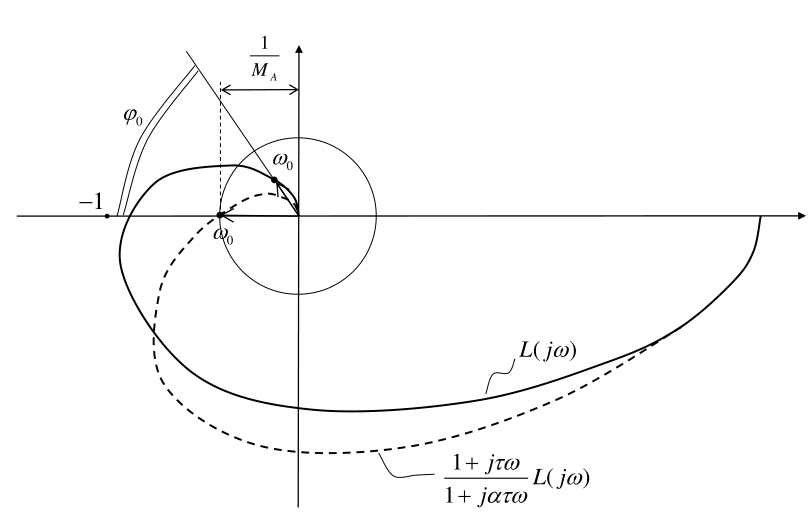
\includegraphics[width=0.5\linewidth]{./images/sintesi_con_margine_ampiezza.png}
  \caption{Sintesi con margine di ampiezza}
  \label{fig:sintesi_con_margine_ampiezza}
\end{figure}


La procedura di sintesi delle rete anticipatrice prevede:
\begin{enumerate}
  \item Scegliere $\omega_0$ affinchè con $\varphi_0 := -\arg L(j\omega_0) -\pi$
    valga $\cos \varphi_0 > M_A |L(j\omega_0)|$
\end{enumerate}

\subsection{Sintesi della rete ritaratrice con imposizione del margine di ampiezza}
\begin{enumerate}
  \item Scegliere $\omega_0$ affinchè con $\varphi_0 := \arg L(j\omega_0) + \pi$
    valga $\cos \varphi_0 > \frac{1}{M_A |L(j\omega_0)|}$

  \item Definiti $M := M_A |L(j\omega_0)|$ e $\varphi := \varphi_0$
    segue che:
    \begin{align}
      \tau &= \frac{M - \cos \varphi}{\omega_0 \sin \varphi} \\
      \alpha &= \frac{M \cos \varphi - 1}{M(M - \cos \varphi)}
    \end{align}
\end{enumerate}


\subsection{La rete a ritardo e anticipo e la rete a T}
Definita dalla formula:
\begin{equation}
  C_r(s) = \frac{1 + 2 \delta' \frac{s}{\omega_n} + \frac{s^2}{\omega_n^2}}{
    1 + 2 \delta \frac{s}{\omega_n} + \frac{s^2}{\omega_n^2}
  }
\end{equation}

Ciò che differenzia le reti e la configurazione di:
\begin{itemize}
  \item Rete a ritarado e anticipo: $\omega_n > 0, \delta > \delta' \geq 1$
  \item Rete a T: $\omega_n > 0, \delta > 1, \delta > \delta' > 0$
\end{itemize}


\subsection{Progetto delle reti con imposizione del margine di fase}

Procedura di sintesi per rete a ritardo e anticipo e rete a T:
\begin{enumerate}
  \item Determinare $\omega_0$ soluzione dell'equazione:
    \begin{equation}
      \arg L()j\omega_0) = -\pi + M_F
    \end{equation}

  \item Imporre:
    \begin{equation}
      \omega_n = \omega_0, \quad \frac{\delta'}{\delta} = \frac{1}{|L(j\omega_0)|}
    \end{equation}
\end{enumerate}

\subsection{Progetto delle reti con imposizione del margine di ampiezza}
Procedura di sintesi per rete a ritardo e anticipo e rete a T:
\begin{enumerate}
  \item Determinare $\omega_p := \arg L(j\omega_p) = -\pi$
  \item Imporre $\omega_n = \omega_p, \quad \frac{\delta'}{\delta} = \frac{1}{M_A |L(j\omega_p)|}$
\end{enumerate}

\subsection{La sintesi con l'equazione diofantea}
Partendo da una funzone di trasferimento razionale:
\begin{equation}
  P(s) := \frac{b(s)}{a(s)} := \frac{b_{n-1}s^{n-1} + \dots + b_0}{s^n + a_{n-1}s^{n-1} + \dots + a_0}
\end{equation}

L'euqazione diofantea è definita come:
\begin{equation}
  a(s)x(s) + b(s)y(s) = d(s)
\end{equation}

\begin{theorem}
  L’equazione diofantea ammette soluzione se e solo se il 
massimo comun divisore di a(s) e b(s) è divisore di d(s)
\end{theorem}

